\scanpage{4}

\diagram{\begin{tikzcd}[ampersand replacement=\&,column sep=1.6em,row sep=1.2ex]
\mathrm{Ob}\,C_4
 \arrow[rr,phantom,"{\tikz[baseline=(current bounding box.center),x=.008cm,y=-.008cm,line cap=round,line join=round]{
  \draw[line width=.8pt] (606,136)--(855,170)--(1027,176);
  \draw[line width=.35pt] (611,163)..controls(650,135)and(850,125)..(1023,174)
   (609,137)--(659,146)--(996,171) (607,136)--(617,145)
   (839,165)--(864,184)
   (844,169)..controls(903,188)and(974,188)..(1021,178)
   (998,151)--(1026,174)--(978,193)
   (994,162)--(1025,173)--(964,203);
  \fill (950,130) circle[radius=1.3];
  \fill (999,162)--(1031,172)--(1008,187)--(1013,174)--cycle;
 }}" description,pos=.54] \& \& \tikz[baseline=(targetF.base)]{
 \node[inner sep=0pt] (targetF) {\(\mathrm{Fl}_0\)};
 \fill ([xshift=-.13em,yshift=.02em]targetF.south west) circle[radius=.025em];}
 (\ell_{\unsure{n|1}})\\
{\tikz[baseline=(topproduct.base)]{
 \node[inner sep=0pt] (topproduct) {\(\bigl(\mathbb F\mathrm l\,C_1\times\mathrm{Ob}\,C_2\bigr)\)};
 \fill ([xshift=1.05em,yshift=-.48em]topproduct.west) circle[radius=.025em];}}
 \arrow[u,phantom,"{\tikz[baseline=(current bounding box.center),x=.008cm,y=-.008cm,line cap=round,line join=round]{
  \draw[line width=.45pt] (286,260)--(289,178) (276,208)--(289,178)--(298,199)
   (284,254)..controls(282,246)and(284,202)..(287,185)
   (286,260)--(292,257) (321,257)--(318,184) (321,257)--(327,254)
   (307,190)--(327,173)--(334,182);
 }}" description,pos=.5]
 \& {\begin{aligned}
 &\deleted{\amalg}\;\deleted{\unsure{\mathrm{Fl}_0 C_1\times}}\\[-.3ex]
 &\qquad\inserted{\mathbb F\mathrm l_0(\ell_1)
 \mathbin{\tikz[baseline=(replacementcross.base)]{
  \node[inner sep=0pt] (replacementcross) {\(\times\)};
  \fill ([xshift=.09em,yshift=.12em]replacementcross.north east) circle[radius=.025em];}}
 \mathrm{Ob}\,C_2}
 \end{aligned}} \&
\end{tikzcd}}
% The heavy arrow certainly points right. Its multiple shafts and left spur
% are traced without asserting a separately cancelled earlier left arrow.
% Detached points have unassigned origin/function; the right upward head is gapped.

\[
\mathbb F\mathrm l\,C_{\deleted{\unsure{2}}\unsure{1|2}}\times
\mathbb F\mathrm l(C_2)\times\deleted{\unsure{F|\mathrm{Fl}}}\mathrm{Ob}\,C_3
\]

\figure{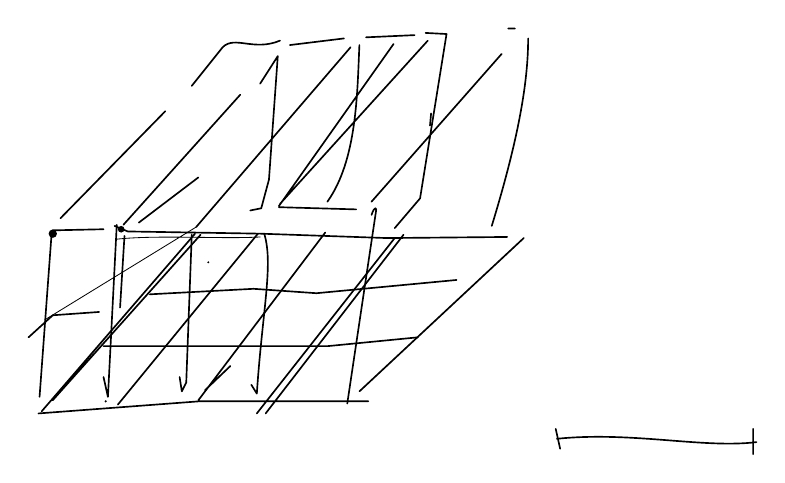
\begin{tikzpicture}[x=.014cm,y=-.014cm,line width=.6pt,line cap=round,line join=round]
\draw (1305,284)--(1351,283) (1361,280)--(1373,285)--(1493,287)--(1608,291)--(1717,290)
 (1304,286)--(1293,435) (1363,279)--(1355,435)--(1351,417) (1370,289)--(1366,354)
 (1431,288)--(1426,422)--(1422,430)--(1420,417)
 (1497,288)..controls(1505,316)and(1495,357)..(1490,432)--(1485,424)
 (1594,270)..controls(1597,261)and(1599,264)..(1598,267)--(1572,441);
\draw[line width=.3pt] (1298,365)--(1435,281)
 (1363,292)..controls(1400,288)and(1460,292)..(1493,290);
\draw (1292,450)--(1438,439)--(1591,439)
 (1295,448)--(1434,287) (1305,438)--(1439,288)
 (1364,442)--(1491,287) (1437,438)--(1552,286) (1443,429)--(1466,407)
 (1490,450)--(1615,291) (1498,450)--(1623,288) (1583,430)--(1732,291);
\draw (1283,381)--(1305,361)--(1347,358) (1351,389)--(1554,389)--(1636,381)
 (1393,342)--(1487,337)--(1544,341)--(1671,329);
\draw (1312,273)--(1407,176) (1369,279)--(1475,161) (1383,277)--(1437,236)
 (1431,153)--(1459,118)..controls(1470,107)and(1487,122)..(1511,112)
 (1493,151)--(1509,126)--(1501,238)--(1494,264)--(1484,266)
 (1520,116)--(1569,110) (1435,281)--(1575,118)
 (1510,262)--(1614,115) (1510,263)--(1580,265)
 (1554,258)..controls(1581,220)and(1581,159)..(1583,116)
 (1589,109)--(1633,107) (1511,260)--(1645,112)
 (1643,105)--(1662,106)--(1638,255)--(1615,282)
 (1594,258)--(1712,124) (1703,280)..controls(1725,208)and(1736,154)..(1736,110);
\fill (1305,287) circle[radius=3.8] (1367,283) circle[radius=3];
\draw (1718,101)--(1724,101) (1648,178)--(1647,189);
\fill (1353,439) circle[radius=1.1] (1446,313) circle[radius=1.0];
% The detached dash and two small points are traced without assigning meaning.
\draw (1762,473)..controls(1830,466)and(1895,482)..(1943,476)
 (1761,464)--(1765,482) (1940,464)--(1940,487);
\end{tikzpicture}}

\[
\mathbb F_3=\mathrm{Fl}\,C_1\times\mathrm{Fl}\,C_2
\,<\,\unsure{\mathbb F|F}\mathrm l\,\ell_3\times\mathrm{Ob}\,C_4
\]

\[
\mathbb F_n\mathrel{2}\mathbb F\mathrm l.C_1
<\mathrm{Fl}\,C_2\ \text{---}\ \times\mathbb F\mathrm l\,C_n
\deleted{\times\mathrm{Ob}\,C_4}
% The last Fl follows the first candidate of the preceding F-alphabet doubt.
% The small point before C_1 is reproduced without a punctuation assignment.
\]

\figure{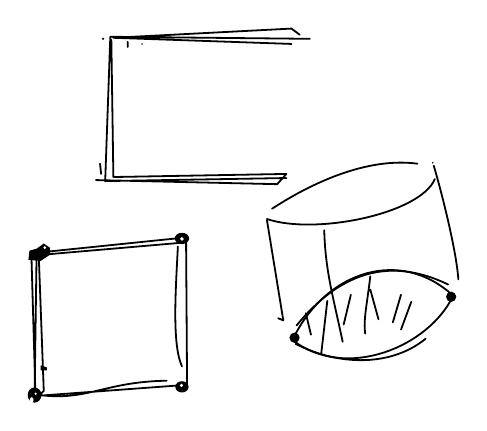
\begin{tikzpicture}[x=.013cm,y=-.013cm,line width=.65pt,line cap=round,line join=round]
\draw (1805,608)--(1610,606)--(1605,747)--(1782,744)
 (1795,604)--(1787,598)--(1613,607)--(1787,613)
 (1611,609)--(1613,743) (1596,746)--(1773,750)--(1782,740)--(1614,743);
\fill (1603,608) circle[radius=1.2] (1641,613) circle[radius=.8];
\draw (1627,611)--(1627,616) (1600,730)--(1601,740);
\draw (1538,817)--(1684,802)--(1685,946)--(1536,957)--cycle
 (1543,819)--(1682,807) (1533,822)--(1537,960)--(1545,952)--(1540,817)
 (1676,811)..controls(1674,852)and(1670,906)..(1680,928)
 (1541,956)..controls(1588,962)and(1604,943)..(1665,942);
\fill (1531,815)--(1538,813)--(1545,808)--(1551,812)--(1551,819)
 --(1542,825)--(1530,824)--cycle;
\fill (1680,803) ellipse[x radius=7,y radius=5.5];
\fill (1680,948) ellipse[x radius=6.5,y radius=5.5];
\fill (1536,956) ellipse[x radius=6.7,y radius=7.4];
\fill[white] (1546,812) circle[radius=1.5]
 (1680,803.5) circle[radius=1.9] (1679.5,946.6) circle[radius=1.7]
 (1537.1,954.7) circle[radius=1.25];
\fill[white] (1533.2,960.8) ellipse[x radius=1.8,y radius=2.7];
\fill (1542,927)--(1548,929)--(1548,932)--(1542,932)--cycle;
\draw (1768,774)..controls(1814,744)and(1866,724)..(1910,730)
 (1763,784)..controls(1810,800)and(1913,779)..(1927,745)
 (1763,785)--(1779,883)--(1774,881) (1926,732)..controls(1932,752)and(1948,813)..(1950,843)
 (1819,795)..controls(1820,835)and(1828,861)..(1837,904);
\fill (1925,729) circle[radius=.9];
\draw (1789,900)..controls(1822,834)and(1894,812)..(1945,859)
 ..controls(1921,909)and(1841,942)..(1789,903);
\draw (1792,888)..controls(1832,839)and(1880,819)..(1940,848)
 (1791,906)..controls(1834,928)and(1885,928)..(1918,901);
\draw (1801,876)--(1806,897) (1822,864)--(1816,916) (1845,858)--(1838,887)
 (1864,840)..controls(1861,866)and(1857,883)..(1859,896)
 (1864,853)--(1872,882) (1894,858)--(1886,885) (1904,865)--(1894,892);
\fill (1790,900) circle[radius=5] (1943,860) circle[radius=5];
\end{tikzpicture}}

\[
\tikz[baseline=(markletters.base)]{
 \node[inner sep=0pt] (markletters) {\(\unsure{X_0|X_{\varnothing}}\qquad X_1\)};
 \draw[line width=.32pt] ([xshift=.75em,yshift=-.4em]markletters.west)
 ..controls ([xshift=1.4em,yshift=.5em]markletters.west) and ([xshift=-1.05em,yshift=.6em]markletters.east)
 ..([xshift=-1em,yshift=-.05em]markletters.east)
 ..controls ([xshift=-.95em,yshift=-.6em]markletters.east) and ([xshift=-.5em,yshift=-.5em]markletters.east)
 ..([xshift=-.1em,yshift=0em]markletters.east)
 ..controls ([xshift=.1em,yshift=.2em]markletters.east) and ([xshift=.15em,yshift=.2em]markletters.east)
 ..([xshift=.2em,yshift=-.1em]markletters.east);
 \draw[line width=.25pt] ([xshift=.35em,yshift=.02em]markletters.west)
 --([xshift=.72em,yshift=.5em]markletters.west);
 \draw[line width=.4pt] ([xshift=-.8em,yshift=.95em]markletters.east)
 --([xshift=-.78em,yshift=.85em]markletters.east);}
% The connecting trace and detached upper tick are not assigned an arrow
% or cancellation function. The crossed first index remains uncertain.
\]

\[
\bullet\quad O_1\subset\mathbb F_1\qquad
\deleted{\mathbb F}O_2\subset\mathbb F_2\quad\text{---}\quad O_n\subset
\tikz[baseline=(lastinclusionF.base)]{
 \node[inner sep=0pt] (lastinclusionF) {\(\mathbb F_n\)};
 \fill ([xshift=-.25em,yshift=.09em]lastinclusionF.north west) circle[radius=.023em];}
\]

\[
\tikz[baseline=(rightoverlay.base)]{
 \node[inner sep=0pt] (rightoverlay) {\(\unsure{\deleted{O}\hat{\mathbb F}|\deleted{\mathbb F}\hat O}\)};
 \draw[line width=.3pt] ([xshift=-.16em,yshift=-.1em]rightoverlay.south west)
 --([xshift=-.02em,yshift=.22em]rightoverlay.south west);}
 \subset\mathbb F
% Overlay order is uncertain. The low left slant is literal, with function unassigned.
\]

\[
\mathbb F_1\times\text{---}\,
\mathbin{\tikz[baseline=(tickcross.base)]{
 \node[inner sep=0pt] (tickcross) {\(\times\)};
 \draw[line width=.3pt] ([xshift=.12em,yshift=.36em]tickcross.north)
 ..controls ([xshift=.2em,yshift=.23em]tickcross.north) and ([xshift=.18em,yshift=.13em]tickcross.north)
 ..([xshift=.08em,yshift=.08em]tickcross.north);}}
\mathbb F_n
\mathbin{\tikz[baseline=(dotcross.base)]{
 \node[inner sep=0pt] (dotcross) {\(\times\)};
 \fill ([xshift=.12em,yshift=.12em]dotcross.north east) circle[radius=.45pt];}}
(-\,?)
% Detached curved tick above the second cross and dot above-right of the
% third cross are reproduced literally; their linguistic status is unknown.
\]

\[
(O_1,\mathbb F_1
\tikz[baseline=(pairclose.base)]{
 \node[inner sep=0pt] (pairclose) {\()\)};
 \draw[line width=.3pt] ([xshift=-.02em,yshift=.04em]pairclose.center)
 --([xshift=-.22em,yshift=-.2em]pairclose.center);}
\mathbin{*}(O_2,\mathbb F_2)\ 
\tikz[baseline=(pairdash.base)]{
 \node[inner sep=0pt] (pairdash) {\(\text{---}\)};
 \fill ([xshift=-.25em,yshift=.08em]pairdash.west) ellipse[x radius=.02em,y radius=.04em];}
\mathbin{*}
(\deleted{\unsure{O|0}}\unsure{O_3|O_n}\,\unsure{F_n|F_{n+1}|F_3})\,.
\]

\figure{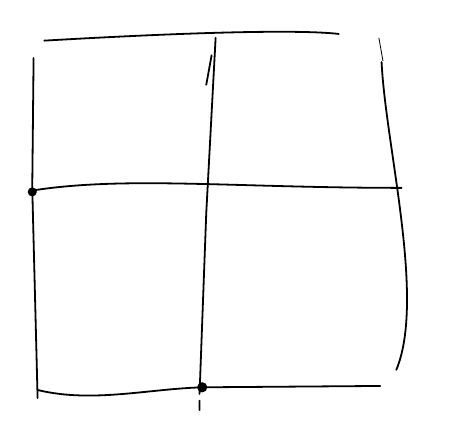
\begin{tikzpicture}[x=.017cm,y=-.017cm,line width=.65pt,line cap=round]
\draw (1374,1202)..controls(1460,1197)and(1559,1193)..(1594,1197)
 (1366,1215)--(1365,1312)--(1369,1469)
 (1365,1314)..controls(1435,1303)and(1515,1312)..(1641,1312)
 (1502,1200)--(1495,1331)--(1490,1466) (1490,1471)--(1490,1478)
 (1499,1213)--(1495,1235)
 (1369,1463)..controls(1410,1473)and(1452,1462)..(1493,1461)--(1625,1460)
 (1626,1218)..controls(1629,1281)and(1659,1395)..(1637,1448);
\draw[line width=.3pt] (1624,1200)--(1627,1217);
\fill (1365,1315) circle[radius=3.4] (1492,1461) circle[radius=3.8];
\end{tikzpicture}}

\[
(F\times I)\mathbin{\amalg}_{\unsure{\deleted{O}\dot{\mathbb F}|\dot B}\times I}
\deleted{O}\hat{\mathbb F}
% The final overlay follows the first candidate of the earlier order doubt.
% The small subscript composite retains a separate B alternative.
\]
% archive sheet number: 3
